\newcommand{\drawblock}[4]{% Parameters: color, stack, level,  label
  \draw[draw=black,fill=#1!55] (#2,0.8*#3) ++(0,0.8) -- ++(0.8,0) -- ++(0.4,0.4) -- ++(-0.8,0) -- ++(-0.4,-0.4);
  \draw[draw=black,fill=#1!75] (#2,0.8*#3) ++(0.8,0) -- ++(0.4,0.4) -- ++(0,0.8) -- ++(-0.4,-0.4) -- ++(0,-0.8);
  \draw[draw=black,fill=#1]    (#2,0.8*#3) rectangle +(0.8,0.8);
  \path (#2,0.8*#3) +(0.4,0.4) node {#4};
}

\newcommand{\drawblackblock}[3]{% Parameters: stack, level,  label
  \draw[draw=black!90!white,fill=blue!10!white] (#1,0.8*#2) ++(0,0.8) -- ++(0.8,0) -- ++(0.4,0.4) -- ++(-0.8,0) -- ++(-0.4,-0.4);
  \draw[draw=black!90!white,fill=blue!10!white] (#1,0.8*#2) ++(0.8,0) -- ++(0.4,0.4) -- ++(0,0.8) -- ++(-0.4,-0.4) -- ++(0,-0.8);
  \draw[draw=black!90!white,fill=blue!10!white] (#1,0.8*#2) rectangle +(0.8,0.8);
  \path (#1,0.8*#2) +(0.4,0.4) node {#3};
}

\newcommand{\drawtable}[1]{ % Parameter: number of stacks
  \draw[draw=black!80!white,fill=black!50!white] (-0.2,-0.2) -- ++(#1,0) -- ++(0.2,0)
  -- ++(0.8,0.8) -- ++(-0.2,0) -- ++(-#1,0) -- ++(-0.2,0) -- ++(-0.8,-0.8) -- ++(0.2,0);
} 

\newcommand{\drawleftfinger}[2]{ % Parameters: stack, level
  \draw[draw=black!80!white,fill=black!50!white] (#1,0.8*#2) ++(0.1,0.5) -- ++(0.2,0.2)
  -- ++(0,0.6) -- ++(-0.2,-0.2) -- ++(0,-0.6);
  \draw[draw=black!80!white,fill=black!50!white] (#1,0.8*#2) ++(-0.1,0.5) rectangle +(0.2,0.6);
}

\newcommand{\drawrightfinger}[2]{ % Parameters: stack, level
  \draw[draw=black!80!white,fill=black!50!white] (#1,0.8*#2) ++(1.1,0.5) -- ++(0.2,0.2)
  -- ++(0,0.6) -- ++(-0.2,-0.2) -- ++(0,-0.6);
  \draw[draw=black!80!white,fill=black!50!white] (#1,0.8*#2) ++(0.9,0.5) rectangle +(0.2,0.6);
}

\newcommand{\drawhandfront}[2]{ % Parameters: stack, level
  \draw[draw=black!80!white,fill=black!50!white] (#1,0.8*#2) ++(-0.1,0.9) rectangle ++(1.2,0.2);
  \draw[draw=black!50!white,thick] (#1,0.8*#2) ++(-0.095,0.9) -- ++(0.17,0);
  \draw[draw=black!50!white,thick] (#1,0.8*#2) ++(0.91,0.9) -- ++(0.185,0);
}

\newcommand{\drawhandtop}[2]{ % Parameters: stack, level
  \draw[draw=black!80!white,fill=black!50!white] (#1,0.8*#2) ++(-0.1,1.1) -- ++(1.2,0)
  -- ++(0.2,0.2) -- ++(-1.2,0) -- ++(-0.2,-0.2);
}

\newcommand{\drawhandle}[2]{ % Parameters: stack, level
  \draw[draw=black!80!white,fill=black!50!white] (#1,0.8*#2) ++(0.7,1.1) -- ++(0.2,0.2)
  -- ++(0,0.5) -- ++(-0.2,-0.2) --++(0,-0.5);
  \draw[draw=black!80!white,fill=black!50!white] (#1,0.8*#2) ++(0.3,1.6) -- ++(0.4,0)
  -- ++(0.2,0.2) -- ++(-0.4,0) -- ++(-0.2,-0.2);
  \draw[draw=black!80!white,fill=black!50!white] (#1,0.8*#2) ++(0.3,1.1) rectangle ++(0.4,0.5);
  \draw[draw=black!50!white,thick] (#1,0.8*#2) ++(0.305,1.1) -- ++(0.39,0);
}

\newcommand{\drawblackleftfinger}[2]{ % Parameters: stack, level
  \draw[draw=black!90!white,fill=blue!10!white] (#1,0.8*#2) ++(0.1,0.5) -- ++(0.2,0.2)
  -- ++(0,0.6) -- ++(-0.2,-0.2) -- ++(0,-0.6);
  \draw[draw=black!90!white,fill=blue!10!white] (#1,0.8*#2) ++(-0.1,0.5) rectangle +(0.2,0.6);
}

\newcommand{\drawblackrightfinger}[2]{ % Parameters: stack, level
  \draw[draw=black!90!white,fill=blue!10!white] (#1,0.8*#2) ++(1.1,0.5) -- ++(0.2,0.2)
  -- ++(0,0.6) -- ++(-0.2,-0.2) -- ++(0,-0.6);
  \draw[draw=black!90!white,fill=blue!10!white] (#1,0.8*#2) ++(0.9,0.5) rectangle +(0.2,0.6);
}

\newcommand{\drawblackhandfront}[2]{ % Parameters: stack, level
  \draw[draw=black!90!white,fill=blue!10!white] (#1,0.8*#2) ++(-0.1,0.9) rectangle ++(1.2,0.2);
  \draw[draw=blue!10!white, thick] (#1,0.8*#2) ++(-0.095,0.9) -- ++(0.17,0);
  \draw[draw=blue!10!white, thick] (#1,0.8*#2) ++(0.91,0.9) -- ++(0.185,0);
}

\newcommand{\drawblackhandtop}[2]{ % Parameters: stack, level
  \draw[draw=black!90!white,fill=blue!10!white] (#1,0.8*#2) ++(-0.1,1.1) -- ++(1.2,0)
  -- ++(0.2,0.2) -- ++(-1.2,0) -- ++(-0.2,-0.2);
}

\newcommand{\drawblackhandle}[2]{ % Parameters: stack, level
  \draw[draw=black!90!white,fill=blue!10!white] (#1,0.8*#2) ++(0.7,1.1) -- ++(0.2,0.2)
  -- ++(0,0.5) -- ++(-0.2,-0.2) --++(0,-0.5);
  \draw[draw=black!90!white,fill=blue!10!white] (#1,0.8*#2) ++(0.3,1.6) -- ++(0.4,0)
  -- ++(0.2,0.2) -- ++(-0.4,0) -- ++(-0.2,-0.2);
  \draw[draw=black!90!white,fill=blue!10!white] (#1,0.8*#2) ++(0.3,1.1) rectangle ++(0.4,0.5);
  \draw[draw=blue!10!white,thick] (#1,0.8*#2) ++(0.305,1.1) -- ++(0.39,0);
}

\definecolor{Navy}{rgb}{0.3,0.3,1}

\newcommand{\bwstateA}{
  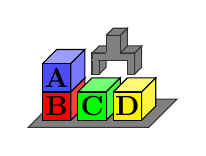
\begin{tikzpicture}[scale=0.45]
    \drawtable{3}
    \drawblock{red}{0}{0}{\textbf{B}}
    \drawblock{Navy}{0}{1}{\textbf{A}}
    \drawblock{green}{1}{0}{\textbf{C}}
    \drawblock{yellow}{2}{0}{\textbf{D}}
    \drawleftfinger{1.5}{1}
    \drawrightfinger{1.5}{1}
    \drawhandfront{1.5}{1}
    \drawhandtop{1.5}{1}
    \drawhandle{1.5}{1}
  \end{tikzpicture}
}

\newcommand{\bwstateB}{
  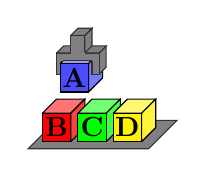
\begin{tikzpicture}[scale=0.45]
    \drawtable{3}
    \drawblock{red}{0}{0}{\textbf{B}}
    \drawblock{green}{1}{0}{\textbf{C}}
    \drawblock{yellow}{2}{0}{\textbf{D}}
    \drawleftfinger{0.5}{1.75}
    \drawblock{Navy}{0.5}{1.75}{\textbf{A}}
    \drawrightfinger{0.5}{1.75}
    \drawhandfront{0.5}{1.75}
    \drawhandtop{0.5}{1.75}
    \drawhandle{0.5}{1.75}
  \end{tikzpicture}
}

\newcommand{\bwstateC}{
  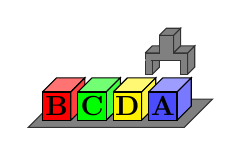
\begin{tikzpicture}[scale=0.45]
    \drawtable{4}
    \drawblock{red}{0}{0}{\textbf{B}}
    \drawblock{green}{1}{0}{\textbf{C}}
    \drawblock{yellow}{2}{0}{\textbf{D}}
    \drawblock{Navy}{3}{0}{\textbf{A}}
    \drawleftfinger{3}{1}
    \drawrightfinger{3}{1}
    \drawhandfront{3}{1}
    \drawhandtop{3}{1}
    \drawhandle{3}{1}
  \end{tikzpicture}
}

\newcommand{\bwstateD}{
  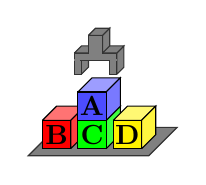
\begin{tikzpicture}[scale=0.45]
    \drawtable{3}
    \drawblock{red}{0}{0}{\textbf{B}}
    \drawblock{green}{1}{0}{\textbf{C}}
    \drawblock{yellow}{2}{0}{\textbf{D}}
    \drawblock{Navy}{1}{1}{\textbf{A}}
    \drawleftfinger{1}{2}
    \drawrightfinger{1}{2}
    \drawhandfront{1}{2}
    \drawhandtop{1}{2}
    \drawhandle{1}{2}
  \end{tikzpicture}
}

\newcommand{\bwstateAabs}{
  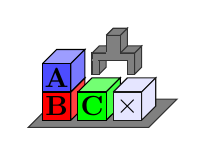
\begin{tikzpicture}[scale=0.45]
    \drawtable{3}
    \drawblock{red}{0}{0}{\textbf{B}}
    \drawblock{Navy}{0}{1}{\textbf{A}}
    \drawblock{green}{1}{0}{\textbf{C}}
    \drawblackblock{2}{0}{\textbf{$\alert{\times}$}}
    \drawleftfinger{1.5}{1}
    \drawrightfinger{1.5}{1}
    \drawhandfront{1.5}{1}
    \drawhandtop{1.5}{1}
    \drawhandle{1.5}{1}
  \end{tikzpicture}
}

\newcommand{\bwstateBabs}{
  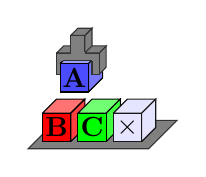
\begin{tikzpicture}[scale=0.45]
    \drawtable{3}
    \drawblock{red}{0}{0}{\textbf{B}}
    \drawblock{green}{1}{0}{\textbf{C}}
    \drawblackblock{2}{0}{\textbf{$\alert{\times}$}}
    \drawleftfinger{0.5}{1.75}
    \drawblock{Navy}{0.5}{1.75}{\textbf{A}}
    \drawrightfinger{0.5}{1.75}
    \drawhandfront{0.5}{1.75}
    \drawhandtop{0.5}{1.75}
    \drawhandle{0.5}{1.75}
  \end{tikzpicture}
}

\newcommand{\bwstateCabs}{
  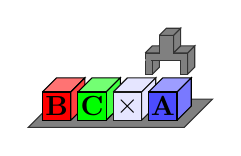
\begin{tikzpicture}[scale=0.45]
    \drawtable{4}
    \drawblock{red}{0}{0}{\textbf{B}}
    \drawblock{green}{1}{0}{\textbf{C}}
    \drawblackblock{2}{0}{\textbf{$\alert{\times}$}}
    \drawblock{Navy}{3}{0}{\textbf{A}}
    \drawleftfinger{3}{1}
    \drawrightfinger{3}{1}
    \drawhandfront{3}{1}
    \drawhandtop{3}{1}
    \drawhandle{3}{1}
  \end{tikzpicture}
}

\newcommand{\bwstateDabs}{
  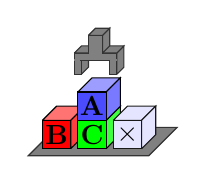
\begin{tikzpicture}[scale=0.45]
    \drawtable{3}
    \drawblock{red}{0}{0}{\textbf{B}}
    \drawblock{green}{1}{0}{\textbf{C}}
    \drawblackblock{2}{0}{\textbf{$\alert{\times}$}}
    \drawblock{Navy}{1}{1}{\textbf{A}}
    \drawleftfinger{1}{2}
    \drawrightfinger{1}{2}
    \drawhandfront{1}{2}
    \drawhandtop{1}{2}
    \drawhandle{1}{2}
  \end{tikzpicture}
}

\newcommand{\blockA}{
  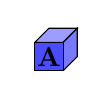
\begin{tikzpicture}[scale=0.45,baseline=2mm]
    \drawblock{Navy}{0}{0}{\textbf{A}}
  \end{tikzpicture}
}

\newcommand{\blockB}{
  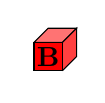
\begin{tikzpicture}[scale=0.45,baseline=2mm]
    \drawblock{red}{0}{0}{\textbf{B}}
  \end{tikzpicture}
}

\newcommand{\blockC}{
  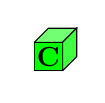
\begin{tikzpicture}[scale=0.45,baseline=2mm]
    \drawblock{green}{0}{0}{\textbf{C}}
  \end{tikzpicture}
}

\newcommand{\blockD}{
  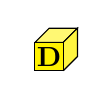
\begin{tikzpicture}[scale=0.45,baseline=2mm]
    \drawblock{yellow}{0}{0}{\textbf{D}}
  \end{tikzpicture}
}

























\newcommand{\bwstateXA}{
  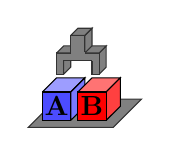
\begin{tikzpicture}[scale=0.45]
    \drawtable{2}
    \drawblock{Navy}{0}{0}{\textbf{A}}
    \drawblock{red}{1}{0}{\textbf{B}}
    \drawleftfinger{0.5}{1}
    \drawrightfinger{0.5}{1}
    \drawhandfront{0.5}{1}
    \drawhandtop{0.5}{1}
    \drawhandle{0.5}{1}
  \end{tikzpicture}
}

\newcommand{\bwstateXB}{
  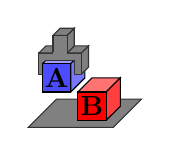
\begin{tikzpicture}[scale=0.45]
    \drawtable{2}
    \drawleftfinger{0}{1}
    \drawblock{Navy}{0}{1}{\textbf{A}}
    \drawrightfinger{0}{1}
    \drawhandfront{0}{1}
    \drawhandtop{0}{1}
    \drawhandle{0}{1}
    \drawblock{red}{1}{0}{\textbf{B}}
  \end{tikzpicture}
}

\newcommand{\bwstateXC}{
  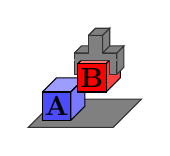
\begin{tikzpicture}[scale=0.45]
    \drawtable{2}
    \drawblock{Navy}{0}{0}{\textbf{A}}
    \drawleftfinger{1}{1}
    \drawblock{red}{1}{1}{\textbf{B}}
    \drawrightfinger{1}{1}
    \drawhandfront{1}{1}
    \drawhandtop{1}{1}
    \drawhandle{1}{1}
  \end{tikzpicture}
}

\newcommand{\bwstateXD}{
  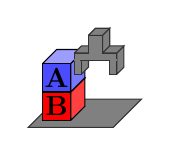
\begin{tikzpicture}[scale=0.45]
    \drawtable{2}
    \drawblock{red}{0}{0}{\textbf{B}}
    \drawblock{Navy}{0}{1}{\textbf{A}}
    \drawleftfinger{1}{1}
    \drawrightfinger{1}{1}
    \drawhandfront{1}{1}
    \drawhandtop{1}{1}
    \drawhandle{1}{1}
  \end{tikzpicture}
}

\newcommand{\bwstateXE}{
  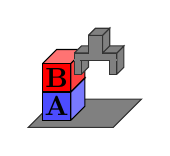
\begin{tikzpicture}[scale=0.45]
    \drawtable{2}
    \drawblock{Navy}{0}{0}{\textbf{A}}
    \drawblock{red}{0}{1}{\textbf{B}}
    \drawleftfinger{1}{1}
    \drawrightfinger{1}{1}
    \drawhandfront{1}{1}
    \drawhandtop{1}{1}
    \drawhandle{1}{1}
  \end{tikzpicture}
}

\newcommand{\bwstateXAabs}{
  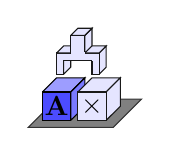
\begin{tikzpicture}[scale=0.45]
    \drawtable{2}
    \drawblock{Navy}{0}{0}{\textbf{A}}
    \drawblackblock{1}{0}{\textbf{$\alert{\times}$}}
    \drawblackleftfinger{0.5}{1}
    \drawblackrightfinger{0.5}{1}
    \drawblackhandfront{0.5}{1}
    \drawblackhandtop{0.5}{1}
    \drawblackhandle{0.5}{1}
  \end{tikzpicture}
}

\newcommand{\bwstateXBabs}{
  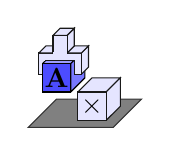
\begin{tikzpicture}[scale=0.45]
    \drawtable{2}
    \drawblackleftfinger{0}{1}
    \drawblock{Navy}{0}{1}{\textbf{A}}
    \drawblackrightfinger{0}{1}
    \drawblackhandfront{0}{1}
    \drawblackhandtop{0}{1}
    \drawblackhandle{0}{1}
    \drawblackblock{1}{0}{\textbf{$\alert{\times}$}}
  \end{tikzpicture}
}

\newcommand{\bwstateXCabs}{
  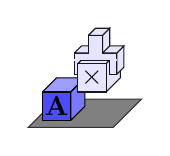
\begin{tikzpicture}[scale=0.45]
    \drawtable{2}
    \drawblock{Navy}{0}{0}{\textbf{A}}
    \drawblackleftfinger{1}{1}
    \drawblackblock{1}{1}{\textbf{$\alert{\times}$}}
    \drawblackrightfinger{1}{1}
    \drawblackhandfront{1}{1}
    \drawblackhandtop{1}{1}
    \drawblackhandle{1}{1}
  \end{tikzpicture}
}

\newcommand{\bwstateXDabs}{
  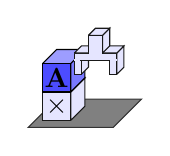
\begin{tikzpicture}[scale=0.45]
    \drawtable{2}
    \drawblackblock{0}{0}{\textbf{$\alert{\times}$}}
    \drawblock{Navy}{0}{1}{\textbf{A}}
    \drawblackleftfinger{1}{1}
    \drawblackrightfinger{1}{1}
    \drawblackhandfront{1}{1}
    \drawblackhandtop{1}{1}
    \drawblackhandle{1}{1}
  \end{tikzpicture}
}

\newcommand{\bwstateXEabs}{
  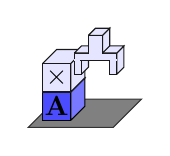
\begin{tikzpicture}[scale=0.45]
    \drawtable{2}
    \drawblock{Navy}{0}{0}{\textbf{A}}
    \drawblackblock{0}{1}{\textbf{$\alert{\times}$}}
    \drawblackleftfinger{1}{1}
    \drawblackrightfinger{1}{1}
    \drawblackhandfront{1}{1}
    \drawblackhandtop{1}{1}
    \drawblackhandle{1}{1}
  \end{tikzpicture}
}



\newcommand{\bwstateYAabs}{
  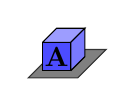
\begin{tikzpicture}[scale=0.45]
    \drawtable{1}
    \drawblock{Navy}{0}{0}{\textbf{A}}
  \end{tikzpicture}
}

\newcommand{\bwstateYBabs}{
  
\begin{tikzpicture}[scale=0.45]
    \drawblackleftfinger{0}{0}
    \drawblock{Navy}{0}{0}{\textbf{A}}
    \drawblackrightfinger{0}{0}
    \drawblackhandfront{0}{0}
    \drawblackhandtop{0}{0}
    \drawblackhandle{0}{0}
  \end{tikzpicture}
}

\newcommand{\bwstateYDabs}{
  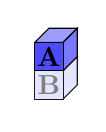
\begin{tikzpicture}[scale=0.45]
    \drawblackblock{0}{0}{{\color{gray}\textbf{B}}}
    \drawblock{Navy}{0}{1}{\textbf{A}}
  \end{tikzpicture}
}
